%%%%%%%%%%%%%%%%%%%%%%%%%%%%%%%%%%%%%%%%%
% Dreuw & Deselaer's Poster
% LaTeX Template
% Version 1.0 (11/04/13)
%
% Created by:
% Philippe Dreuw and Thomas Deselaers
% http://www-i6.informatik.rwth-aachen.de/~dreuw/latexbeamerposter.php
%
% This template has been downloaded from:
% http://www.LaTeXTemplates.com
%
% License:
% CC BY-NC-SA 3.0 (http://creativecommons.org/licenses/by-nc-sa/3.0/)
%
%%%%%%%%%%%%%%%%%%%%%%%%%%%%%%%%%%%%%%%%%

%----------------------------------------------------------------------------------------
%	PACKAGES AND OTHER DOCUMENT CONFIGURATIONS
%----------------------------------------------------------------------------------------

\documentclass[final,hyperref={pdfpagelabels=false}]{beamer}

\usepackage[orientation=portrait,size=a0,scale=1.4]{beamerposter} % Use the beamerposter package for laying out the poster with a portrait orientation and an a0 paper size

\usepackage[utf8]{inputenc} % Enable åäö

\usetheme{I6pd2} % Use the I6pd2 theme supplied with this template

\usepackage[english]{babel} % English language/hyphenation

\usepackage{amsmath,amsthm,amssymb,latexsym} % For including math equations, theorems, symbols, etc

%\usepackage{times}\usefonttheme{professionalfonts}  % Uncomment to use Times as the main font
\usefonttheme[onlymath]{serif} % Uncomment to use a Serif font within math environments

\boldmath % Use bold for everything within the math environment

\usepackage{booktabs} % Top and bottom rules for tables

\graphicspath{{figures/}} % Location of the graphics files

%--------------------------- added packages ---------------------------------------------
\usepackage{caption}
\usepackage{subcaption}
\usepackage{float}

%----------------------------------------------------------------------------------------


%\usecaptiontemplate{\small\structure{\insertcaptionname \insertcaptionnumber: }\insertcaption} % A fix for figure numbering
\usecaptiontemplate{\insertcaptionname ~\insertcaptionnumber: \insertcaption}
\usepackage[labelformat=empty]{caption}		% (tack Häger!)
\usepackage[labelformat=empty]{subcaption} % Removes autolabelstuff, label manually!
%----------------------------------------------------------------------------------------
%	TITLE SECTION 
%----------------------------------------------------------------------------------------

\title{\huge Kitchen Occupation} % Poster title

\author{People counting using depth sensors.} % Author(s)

\institute{Department of Electrical Engineering, Linköping University} % Institution(s)

%----------------------------------------------------------------------------------------
%	FOOTER TEXT
%----------------------------------------------------------------------------------------

\newcommand{\leftfoot}{
\vspace*{-0.004\textheight}
\begin{tabular*}{\linewidth}{@{\extracolsep{\fill} } c c c c c c c}
Erik Fall & Gustav Häger & Malin Rudin & Alexander Sjöholm & Martin Svensson & Mattias Tiger & Nikolaus West
\end{tabular*}

} % Left footer text

\newcommand{\rightfoot}{} %{http://www.densekitchen.bloip.se} % Right footer text



\begin{document}

\addtobeamertemplate{block end}{}{\vspace*{2ex}} % White space under blocks

\begin{frame}[t] % The whole poster is enclosed in one beamer frame

\vspace*{-0.0072\textheight} % Margin to the header

\begin{columns}[t] % The whole poster consists of two major columns, each of which can be subdivided further with another \begin{columns} block - the [t] argument aligns each column's content to the top

\begin{column}{.025\textwidth}\end{column} % Empty spacer column

\begin{column}{.465\textwidth} % The first column

%----------------------------------------------------------------------------------------
%	OBJECTIVES
%----------------------------------------------------------------------------------------

\begin{block}{Objectives}

\begin{enumerate}
\item Create a system to monitor room usage intensity, primarily focusing on student kitchens.
\item The system needs to be cheap and easy to install and maintain.
\item The system should provide real-time information about room usage intensity.
\end{enumerate}

\end{block}

%----------------------------------------------------------------------------------------
%	INTRODUCTION
%----------------------------------------------------------------------------------------
            
%\begin{block}{Introduction ??}
%
%\begin{itemize}
%\item The Linköping University IT department wants to be able to measure room usage intensity, primarily the student kitchens, but also other spaces. In order enable informed decisions to be made on where to invest in e.g. a new kitchen
%\end{itemize}

%\end{block}

%----------------------------------------------------------------------------------------
%	Hardware setup
%----------------------------------------------------------------------------------------

\begin{block}{System}
	\begin{columns} % Subdivide the first main column
		\begin{column}{.54\textwidth} % The first subdivided column within the first main column
			\begin{itemize}
				\item Hardware setup (figure 1)
				\begin{itemize}
					\item One or several Microsoft Kinect cameras and a computational device with Internet connection is required.
				\end{itemize}
				\item Portability
				\begin{itemize}
					\item Cross platform in the sense that we support most UNIX-like systems and Windows.
				\end{itemize}							
			\end{itemize}
		\end{column}
			
		\begin{column}{.43\textwidth} % The second subdivided column within the first main column
			\centering
			\begin{figure}
				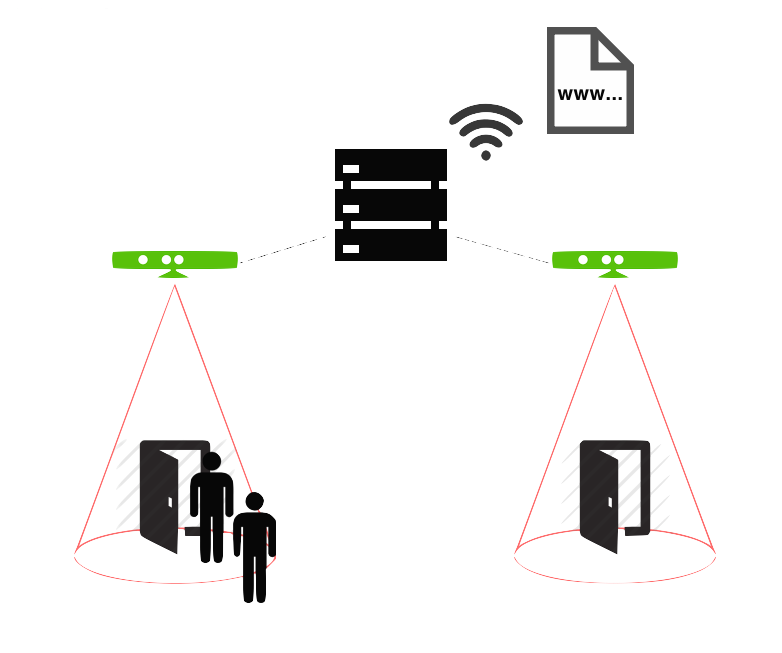
\includegraphics[width=0.9\linewidth]{system_overview.png}
				\caption{\centering \textit{Figure 1:} Rough system overview with main components.}
			\end{figure}
		\end{column}
	\end{columns} % End of the subdivision

\end{block}

%----------------------------------------------------------------------------------------
%	Image Processing
%----------------------------------------------------------------------------------------

\begin{block}{Image Processing Pipeline}
\begin{itemize}
	\item Human segmentation
	\begin{itemize}
	\item Human segmentation is based on the assumption that human heads are distinguishable modes in the depth image and that people moving very close to each other seldom differ radically in height (figure 3). It is realized by a series of threshold and morphological operations, Gaussian blurring, contour drawing and searches for local maxima's (figure 2).
	\end{itemize}
\end{itemize}
\begin{figure}
	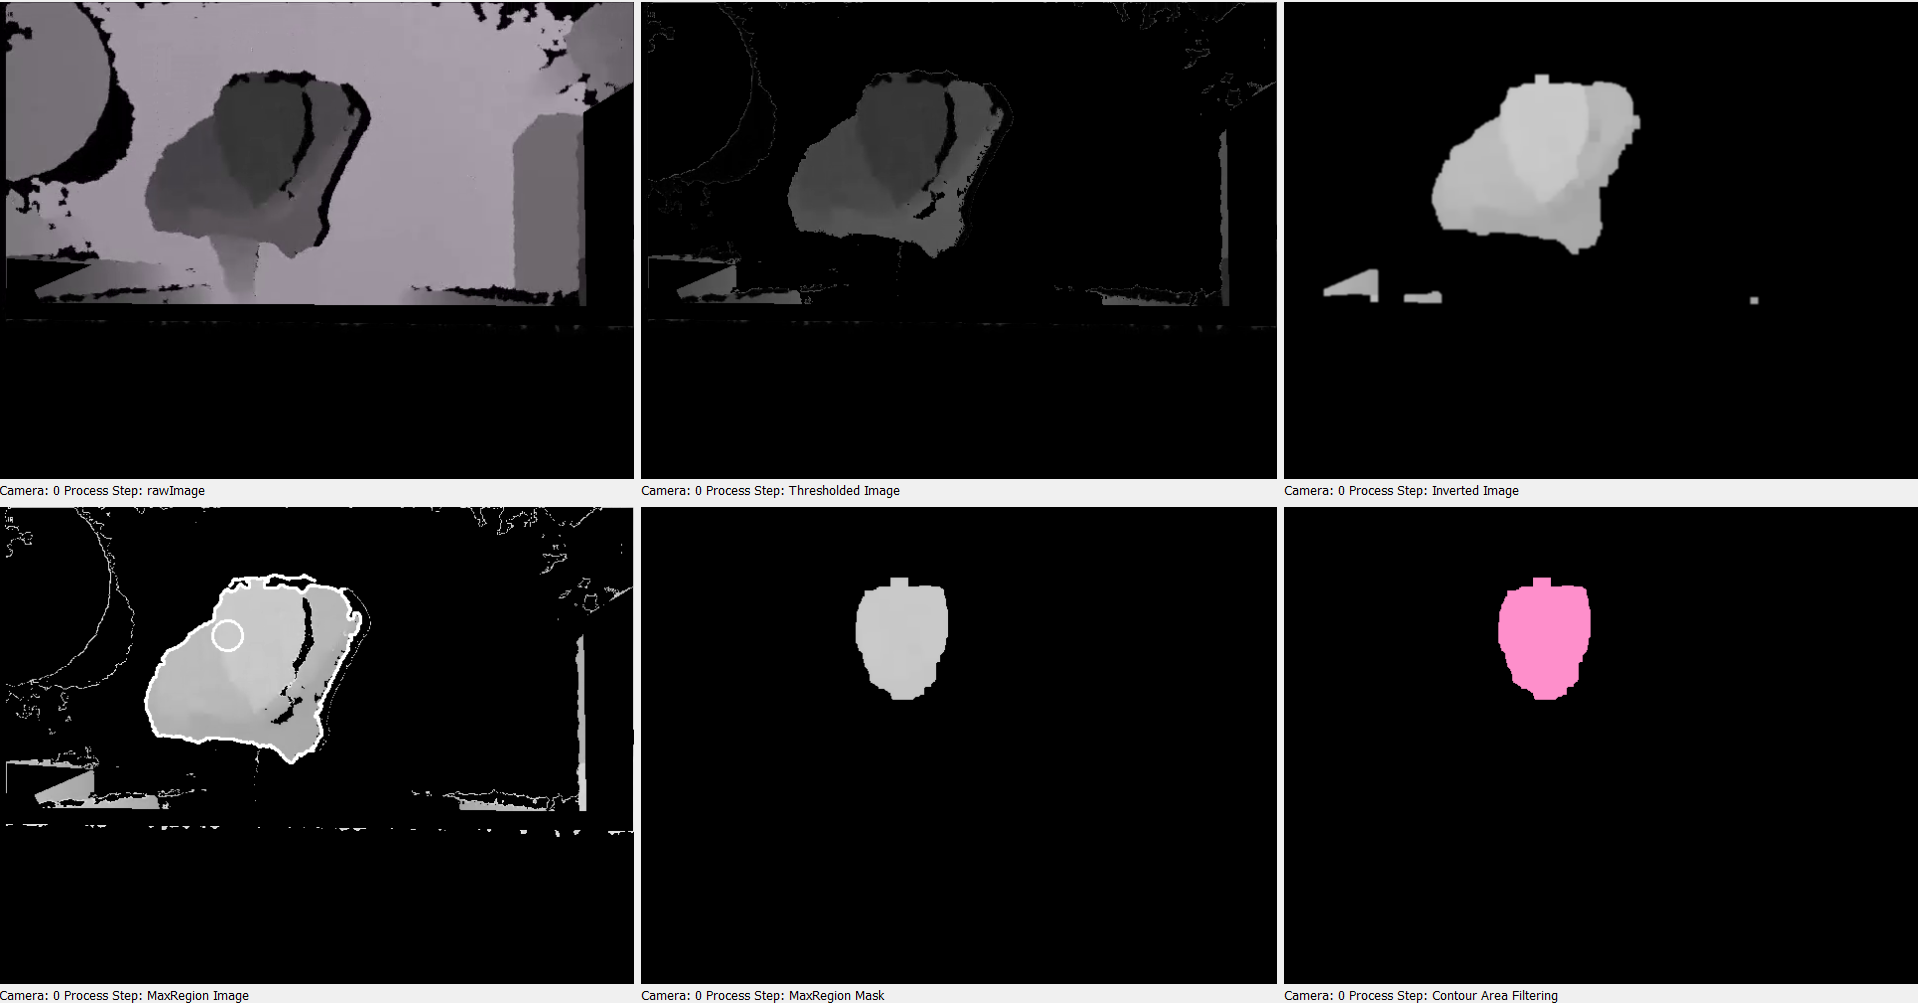
\includegraphics[width=0.9\linewidth]{humanSegmentationSteps.png}
	\caption{\centering \textit{Figure 2:} Top row from the left: Raw input image, Thresholded, Refined depth image. \newline 
			 			 Bottom row from the left: Local Maxima detection, Head thresholding, Segmented heads. }
\end{figure}
\begin{figure}
	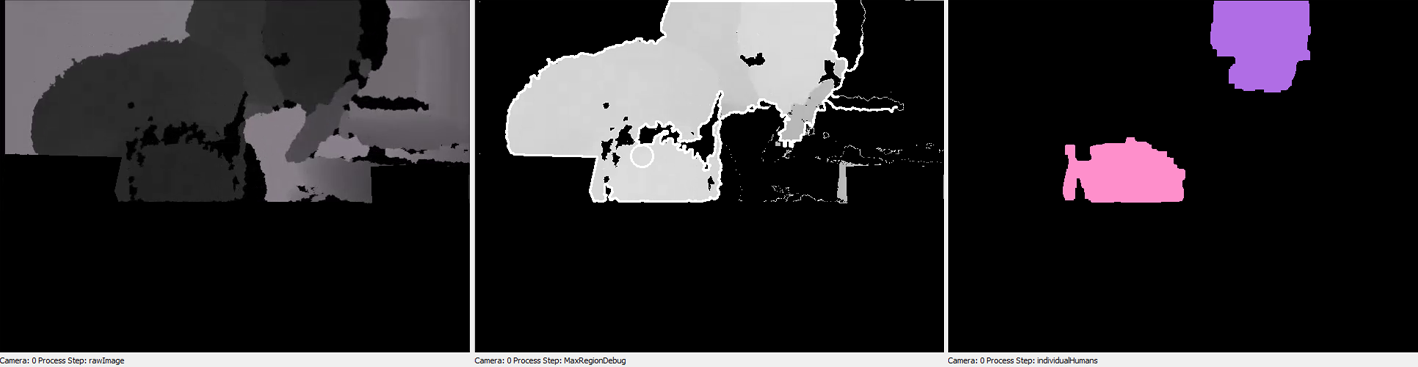
\includegraphics[width=0.9\linewidth]{KinectSegmentationIllustration_occlusionHandling_horizontal.png}
	\caption{\textit{Figure 3:} From left: Raw imput image, Occlusion after thresholding, Successful segmentation}
\end{figure}

\begin{itemize}
	\item Tracking and counting (figure 4)
	\begin{itemize}
		\item{The tracker pairs objects with each other from previous frame to the next. Pairs closest matching objects. Handles occlusion, outliers and noise.}
		\item{Counting is done using user specified checkpoint lines and a door area.}
	\end{itemize}
	
	\item Queue detection (figure 5)
	\begin{itemize}
		\item Objects connected by short Bézier curves, which has been fit to the objects' positions and velocities, are considered in a queue.
		\item Queue severity is determined by queue detection frequency.
	\end{itemize}
\end{itemize}

\begin{figure}
%\centering
\begin{subfigure}{.5\textwidth}
\centering
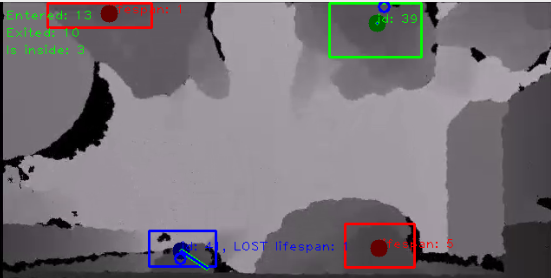
\includegraphics[width=0.9\linewidth]{trackingExample.png}
\caption{\centering \textit{Figure 4:} Newly found potential objects(red), lost 
		 objects(blue) and objects(green)}
\end{subfigure}%
\begin{subfigure}{.5\textwidth}
\centering
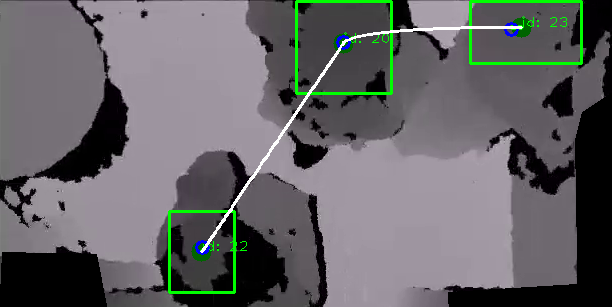
\includegraphics[width=0.9\linewidth]{visibleQueue.png}
\caption{\centering \textit{Figure 5:} A detected queue, illustrated using the spline connecting the persons.}
\end{subfigure}
\end{figure}

\end{block}

%----------------------------------------------------------------------------------------

% ----- NEW COLUMN ---------------------------------------------

\end{column} % End of the first column

\begin{column}{.03\textwidth}\end{column} % Empty spacer column
 
\begin{column}{.465\textwidth} % The second column

% ----- NEW COLUMN ---------------------------------------------




%----------------------------------------------------------------------------------------
%	Software system
%----------------------------------------------------------------------------------------

\begin{block}{Software}
\begin{itemize}
	\item Built in C++ in a very modular, extendable and configurable fashion.
\end{itemize}
	\begin{itemize}
		\item Modular
		\begin{itemize}
			\item Algorithms have a very clear general interface to the rest of the pipeline.
			\item Multiple algorithms of the same type were developed in parallel, with minimal effort on interface compliance.
			\item An entire new computer vision approach could be switched to at the end of the project with minimal effort.
		\end{itemize}
	\end{itemize}
	\begin{itemize}
		\item Configurable
	\begin{itemize}
		\item The entire pipeline can be reconfigured from file. This includes addition, removal and rearrangement of algorithms, and parameter values.
		\item It is possible to automate tests of hundreds of configurations, changing both algorithms and algorithm parameters without re-compiling.
	\end{itemize}
\end{itemize}
\end{block}

%----------------------------------------------------------------------------------------
%	User Interface
%----------------------------------------------------------------------------------------

\begin{block}{Configuration \& Debugging GUI}

\begin{columns} % Subdivide the first main column
\begin{column}{.54\textwidth} % The first subdivided column within the first main column

\begin{itemize}
\item Transparent and flexible pipeline overview (figure 7)
\item Automatic on-line low-level profiling of every module (figure 7)
\item Configuration interface (figure 6)

\begin{itemize}
\item Doors (green)
\item Entering checkpoints (circles)
\item Excluded areas (red)
\end{itemize}
\end{itemize}

\end{column}

\begin{column}{.43\textwidth} % The second subdivided column within the first main column
\centering
\begin{figure}
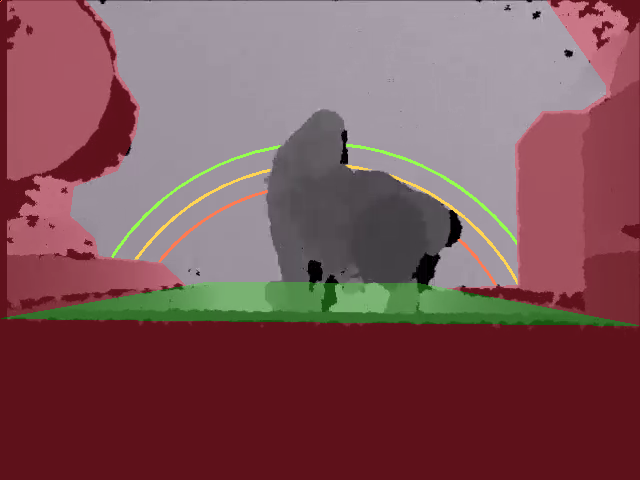
\includegraphics[width=0.985\linewidth]{PosterConfigCrop.png}
\label{fig:Config}
\caption{\textit{Figure 6:} Visualization of configurables}
\end{figure}
\end{column}
\end{columns} % End of the subdivision

\begin{figure}
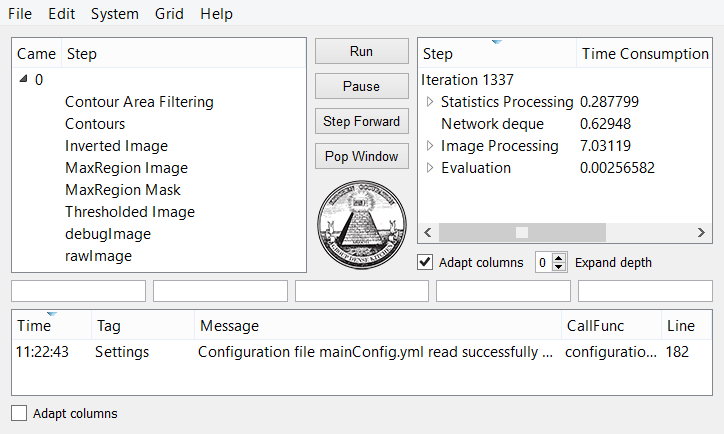
\includegraphics[width=0.9\linewidth]{PosterDebuggerCrop.png}
\caption{\centering \textit{Figure 7:} Main GUI window with the different processing steps, (top left), profiling information (top right) and log messages (bottom)}
\end{figure}

\end{block}


%----------------------------------------------------------------------------------------
%	RESULTS
%----------------------------------------------------------------------------------------


\begin{block}{Results: Table}

\begin{itemize}
\item Final system performance and equations used during evaluation.
\end{itemize}

\begin{equation}
\label{eq:in_accuracy}
A_{in} = 1 - |\frac{\sum_{frames}{in_{Est}}-\sum_{frames}{in_{GT}}}{\sum_{frames}in_{GT}}|
\end{equation} 

\begin{equation}
\label{eq:out_accuracy}
A_{out} = 1 - |\frac{\sum_{frames}{out_{Est}}-\sum_{frames}out_{GT}}{\sum_{frames}out_{GT}}| 
\end{equation} 


\begin{table}[h]
\centering
	\begin{tabular}{r | c | c | c | c | c | c | c }
		\emph{Sequence Name}		&  Total entered (GT) & \emph{$A_{in}$} & Total exited (GT) & \emph{$A_{out}$} & length \\
		\hline \hline
		R-Kitchen			& 108 (108) people & 99 \% & 101 (104) people & 97 \% & 30 min\\
		B25-Kitchen			& 122 (141) people & 87 \% & 77 (91) people & 85 \% & 30 min \\
		U-Kitchen			& 127 (122) people & 96 \% & 136 (135) people & 99 \% & 30 min  \\
		\end{tabular}
	\caption{System performance in the two evaluation sequences}
\end{table}
    
\end{block}

%------------------------------------------------

%\begin{block}{Results: Figure}

%\begin{figure}
%
\includegraphics[width=0.8\linewidth]{placeholder.jpg}
%\caption{Resulting accuracy}
%\end{figure}

%\end{block}

%----------------------------------------------------------------------------------------
%	CONCLUSION
%----------------------------------------------------------------------------------------

\begin{block}{Conclusion}

\begin{itemize}
\item The system provides high-precision real time people counting using the Microsoft Kinect sensor at low computational cost. (2GHz low-end CPU)
\item Very simple assumptions are enough to get good results in practice.
\item The software architecture enables fast implementing and testing of different algorithms. It gives a very lightweight and high-performing vision pipeline.
\end{itemize}
\vspace*{0.0\textheight} % Manual alignment, change this factor if re-alignment is needed.
\end{block}

%----------------------------------------------------------------------------------------
%	REFERENCES
%----------------------------------------------------------------------------------------
%
%\begin{block}{References ??}
%        
%\nocite{*} % Insert publications even if they are not cited in the poster
%\small{\bibliographystyle{unsrt}
%\bibliography{sample}}
%
%\end{block}
%
%%----------------------------------------------------------------------------------------
%%	ACKNOWLEDGEMENTS
%%----------------------------------------------------------------------------------------
%
%\begin{block}{Acknowledgments ?? }
%
%\begin{itemize}
%\item We would like to thank the members of Computer Vision Laboratory here at the university for their endless support and for beign able to provide new sensors and hardware with short notice.
%\end{itemize}
%
%\end{block}

%----------------------------------------------------------------------------------------
%	CONTACT INFORMATION
%----------------------------------------------------------------------------------------

%\setbeamercolor{block title}{fg=black,bg=orange!70} % Change the block title color
%
%\begin{block}{Contact Information}
%
%\begin{itemize}
%\item Web: \href{http://www.university.edu/smithlab}{http://www.university.edu/smithlab}
%\item Email: \href{mailto:john@smith.com}{john@smith.com}
%\item Phone: +1 (000) 111 1111
%\end{itemize}
%
%\end{block}

%----------------------------------------------------------------------------------------

\end{column} % End of the second column

\begin{column}{.02\textwidth}\end{column} % Empty spacer column

\end{columns} % End of all the columns in the poster

\end{frame} % End of the enclosing frame

\end{document}